\documentclass[14pt]{extbook}
\usepackage{multicol, enumerate, enumitem, hyperref, color, soul, setspace, parskip, fancyhdr} %General Packages
\usepackage{amssymb, amsthm, amsmath, latexsym, units, mathtools} %Math Packages
\everymath{\displaystyle} %All math in Display Style
% Packages with additional options
\usepackage[headsep=0.5cm,headheight=12pt, left=1 in,right= 1 in,top= 1 in,bottom= 1 in]{geometry}
\usepackage[usenames,dvipsnames]{xcolor}
\usepackage{dashrule}  % Package to use the command below to create lines between items
\newcommand{\litem}[1]{\item#1\hspace*{-1cm}\rule{\textwidth}{0.4pt}}
\pagestyle{fancy}
\lhead{Progress Quiz 4}
\chead{}
\rhead{Version A}
\lfoot{5346-5907}
\cfoot{}
\rfoot{Summer C 2021}
\begin{document}

\begin{enumerate}
\litem{
Factor the quadratic below. Then, choose the intervals that contain the constants in the form $(ax+b)(cx+d); b \leq d.$\[ 54x^{2} +75 x + 25 \]\begin{enumerate}[label=\Alph*.]
\item \( a \in [17.97, 18.27], \hspace*{5mm} b \in [1, 10], \hspace*{5mm} c \in [2.94, 3.17], \text{ and } \hspace*{5mm} d \in [3, 9] \)
\item \( a \in [2.63, 3.64], \hspace*{5mm} b \in [1, 10], \hspace*{5mm} c \in [17.76, 18.39], \text{ and } \hspace*{5mm} d \in [3, 9] \)
\item \( a \in [7.53, 9.28], \hspace*{5mm} b \in [1, 10], \hspace*{5mm} c \in [5.06, 6.19], \text{ and } \hspace*{5mm} d \in [3, 9] \)
\item \( a \in [0.01, 2.03], \hspace*{5mm} b \in [25, 32], \hspace*{5mm} c \in [0.85, 1.82], \text{ and } \hspace*{5mm} d \in [44, 46] \)
\item \( \text{None of the above.} \)

\end{enumerate} }
\litem{
Write the equation of the graph presented below in the form $f(x)=ax^2+bx+c$, assuming  $a=1$ or $a=-1$. Then, choose the intervals that $a, b,$ and $c$ belong to.
\begin{center}
    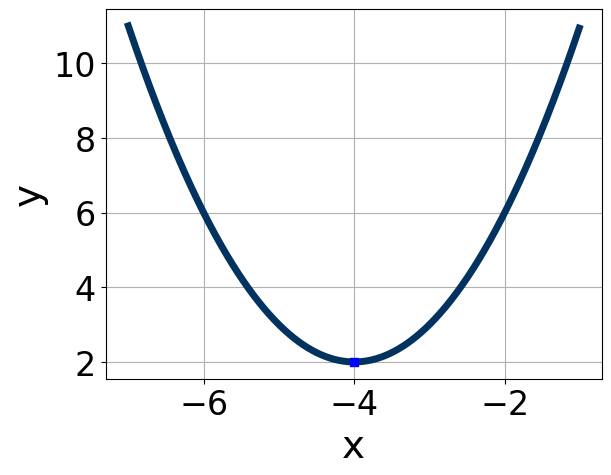
\includegraphics[width=0.5\textwidth]{../Figures/quadraticGraphToEquationA.png}
\end{center}
\begin{enumerate}[label=\Alph*.]
\item \( a \in [1, 3], \hspace*{5mm} b \in [-8, -6], \text{ and } \hspace*{5mm} c \in [17, 19] \)
\item \( a \in [1, 3], \hspace*{5mm} b \in [-8, -6], \text{ and } \hspace*{5mm} c \in [12, 15] \)
\item \( a \in [-2, 0], \hspace*{5mm} b \in [7, 12], \text{ and } \hspace*{5mm} c \in [-15, -13] \)
\item \( a \in [1, 3], \hspace*{5mm} b \in [7, 12], \text{ and } \hspace*{5mm} c \in [17, 19] \)
\item \( a \in [-2, 0], \hspace*{5mm} b \in [-8, -6], \text{ and } \hspace*{5mm} c \in [-15, -13] \)

\end{enumerate} }
\litem{
Factor the quadratic below. Then, choose the intervals that contain the constants in the form $(ax+b)(cx+d); b \leq d.$\[ 24x^{2} +38 x + 15 \]\begin{enumerate}[label=\Alph*.]
\item \( a \in [3.6, 4.3], \hspace*{5mm} b \in [2, 5], \hspace*{5mm} c \in [3.7, 8.4], \text{ and } \hspace*{5mm} d \in [2, 8] \)
\item \( a \in [-2.2, 2.5], \hspace*{5mm} b \in [16, 22], \hspace*{5mm} c \in [0.2, 2.1], \text{ and } \hspace*{5mm} d \in [18, 23] \)
\item \( a \in [4.3, 9.5], \hspace*{5mm} b \in [2, 5], \hspace*{5mm} c \in [2.5, 3.1], \text{ and } \hspace*{5mm} d \in [2, 8] \)
\item \( a \in [-2.2, 2.5], \hspace*{5mm} b \in [2, 5], \hspace*{5mm} c \in [17.7, 21.1], \text{ and } \hspace*{5mm} d \in [2, 8] \)
\item \( \text{None of the above.} \)

\end{enumerate} }
\litem{
Write the equation of the graph presented below in the form $f(x)=ax^2+bx+c$, assuming  $a=1$ or $a=-1$. Then, choose the intervals that $a, b,$ and $c$ belong to.
\begin{center}
    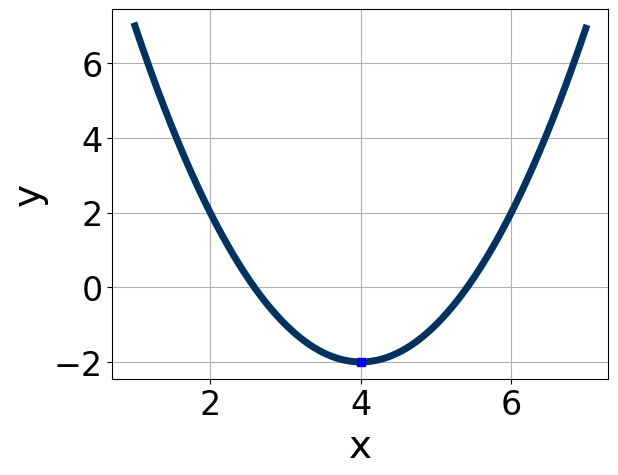
\includegraphics[width=0.5\textwidth]{../Figures/quadraticGraphToEquationCopyA.png}
\end{center}
\begin{enumerate}[label=\Alph*.]
\item \( a \in [0, 3], \hspace*{5mm} b \in [-11, -7], \text{ and } \hspace*{5mm} c \in [12, 16] \)
\item \( a \in [0, 3], \hspace*{5mm} b \in [7, 10], \text{ and } \hspace*{5mm} c \in [12, 16] \)
\item \( a \in [-1, 0], \hspace*{5mm} b \in [7, 10], \text{ and } \hspace*{5mm} c \in [-18, -17] \)
\item \( a \in [0, 3], \hspace*{5mm} b \in [7, 10], \text{ and } \hspace*{5mm} c \in [17, 20] \)
\item \( a \in [-1, 0], \hspace*{5mm} b \in [-11, -7], \text{ and } \hspace*{5mm} c \in [-18, -17] \)

\end{enumerate} }
\litem{
Solve the quadratic equation below. Then, choose the intervals that the solutions belong to, with $x_1 \leq x_2$ (if they exist).\[ -19x^{2} -10 x + 3 = 0 \]\begin{enumerate}[label=\Alph*.]
\item \( x_1 \in [-0.47, 1] \text{ and } x_2 \in [0.36, 0.79] \)
\item \( x_1 \in [-18.58, -17.34] \text{ and } x_2 \in [17.55, 18.46] \)
\item \( x_1 \in [-5.15, -3.78] \text{ and } x_2 \in [13.22, 15.05] \)
\item \( x_1 \in [-1.53, -0.48] \text{ and } x_2 \in [-0.67, 0.65] \)
\item \( \text{There are no Real solutions.} \)

\end{enumerate} }
\litem{
Graph the equation below.\[ f(x) = (x+2)^2 + 10 \]\begin{enumerate}[label=\Alph*.]
\begin{multicols}{2}\item 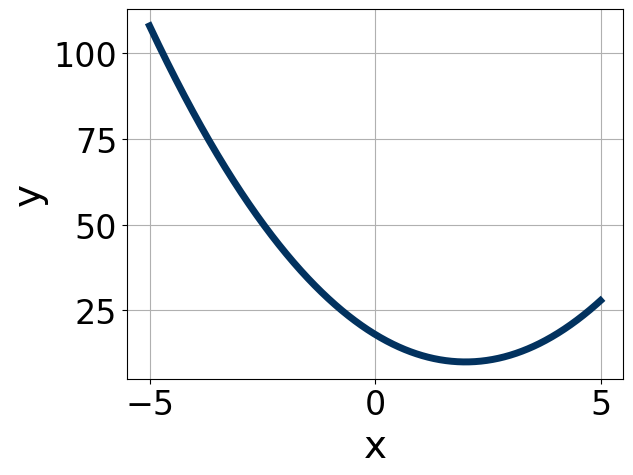
\includegraphics[width = 0.3\textwidth]{../Figures/quadraticEquationToGraphCopyAA.png}\item 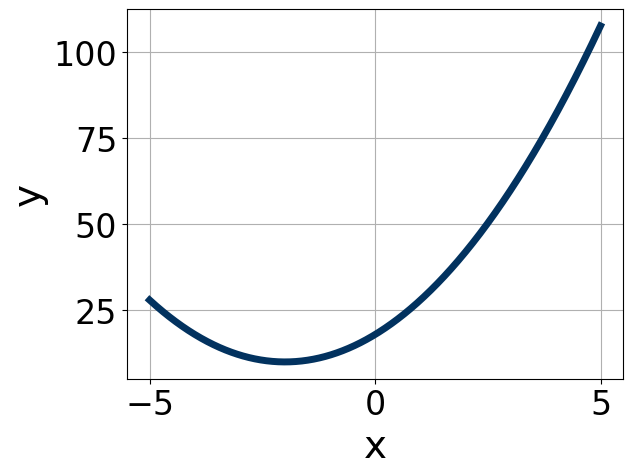
\includegraphics[width = 0.3\textwidth]{../Figures/quadraticEquationToGraphCopyBA.png}\item 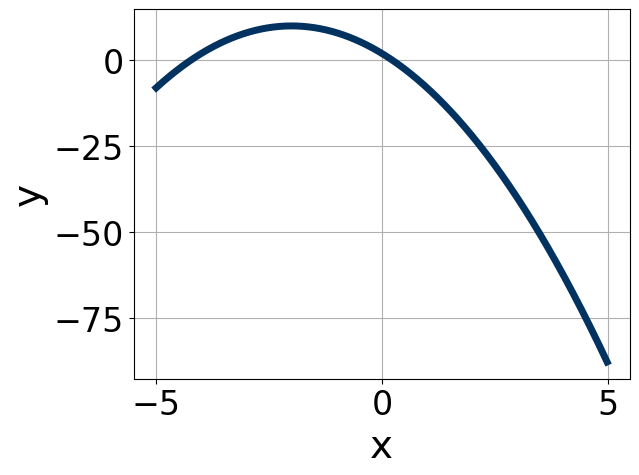
\includegraphics[width = 0.3\textwidth]{../Figures/quadraticEquationToGraphCopyCA.png}\item 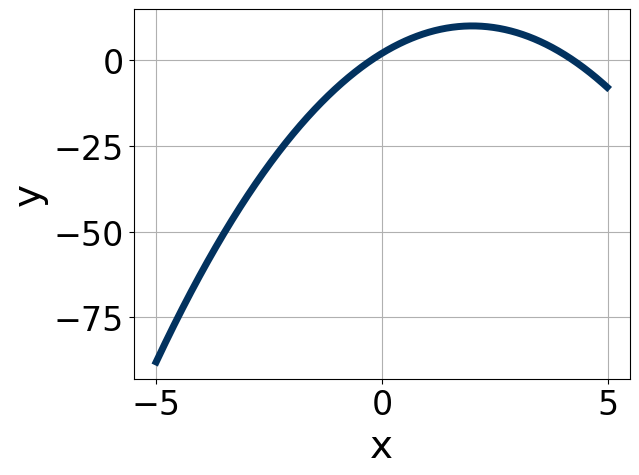
\includegraphics[width = 0.3\textwidth]{../Figures/quadraticEquationToGraphCopyDA.png}\end{multicols}\item None of the above.
\end{enumerate} }
\litem{
Solve the quadratic equation below. Then, choose the intervals that the solutions belong to, with $x_1 \leq x_2$ (if they exist).\[ -15x^{2} -13 x + 4 = 0 \]\begin{enumerate}[label=\Alph*.]
\item \( x_1 \in [-0.3, 0.4] \text{ and } x_2 \in [0.4, 2.8] \)
\item \( x_1 \in [-1.4, -0.91] \text{ and } x_2 \in [0, 1] \)
\item \( x_1 \in [-21.08, -19.8] \text{ and } x_2 \in [19.5, 20.1] \)
\item \( x_1 \in [-3.72, -3.56] \text{ and } x_2 \in [15.5, 17.7] \)
\item \( \text{There are no Real solutions.} \)

\end{enumerate} }
\litem{
Solve the quadratic equation below. Then, choose the intervals that the solutions $x_1$ and $x_2$ belong to, with $x_1 \leq x_2$.\[ 15x^{2} -2 x -24 = 0 \]\begin{enumerate}[label=\Alph*.]
\item \( x_1 \in [-1.34, -0.52] \text{ and } x_2 \in [1.19, 1.54] \)
\item \( x_1 \in [-18.42, -16.06] \text{ and } x_2 \in [19.15, 22.14] \)
\item \( x_1 \in [-0.61, 0.88] \text{ and } x_2 \in [3.23, 4.34] \)
\item \( x_1 \in [-3.25, -1.8] \text{ and } x_2 \in [0.52, 0.91] \)
\item \( x_1 \in [-7.68, -4.82] \text{ and } x_2 \in [-0.11, 0.28] \)

\end{enumerate} }
\litem{
Solve the quadratic equation below. Then, choose the intervals that the solutions $x_1$ and $x_2$ belong to, with $x_1 \leq x_2$.\[ 20x^{2} +21 x -54 = 0 \]\begin{enumerate}[label=\Alph*.]
\item \( x_1 \in [-2.36, -1.61] \text{ and } x_2 \in [0.71, 1.78] \)
\item \( x_1 \in [-45.17, -43.41] \text{ and } x_2 \in [23.82, 24.07] \)
\item \( x_1 \in [-1.74, -0.72] \text{ and } x_2 \in [2.86, 3.92] \)
\item \( x_1 \in [-6.09, -3.29] \text{ and } x_2 \in [0.49, 1.1] \)
\item \( x_1 \in [-9.23, -8.95] \text{ and } x_2 \in [-0.1, 0.31] \)

\end{enumerate} }
\litem{
Graph the equation below.\[ f(x) = -(x-3)^2 - 13 \]\begin{enumerate}[label=\Alph*.]
\begin{multicols}{2}\item 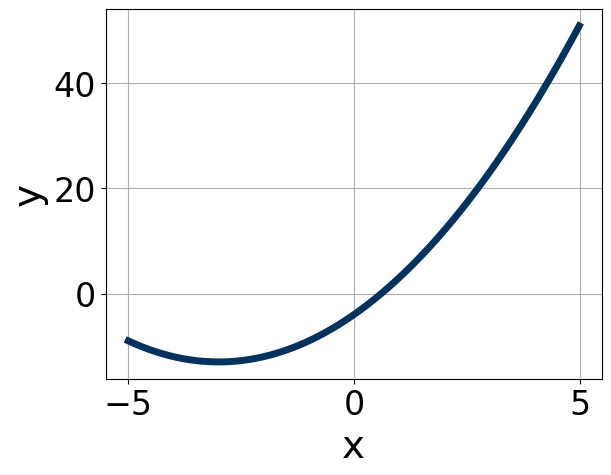
\includegraphics[width = 0.3\textwidth]{../Figures/quadraticEquationToGraphAA.png}\item 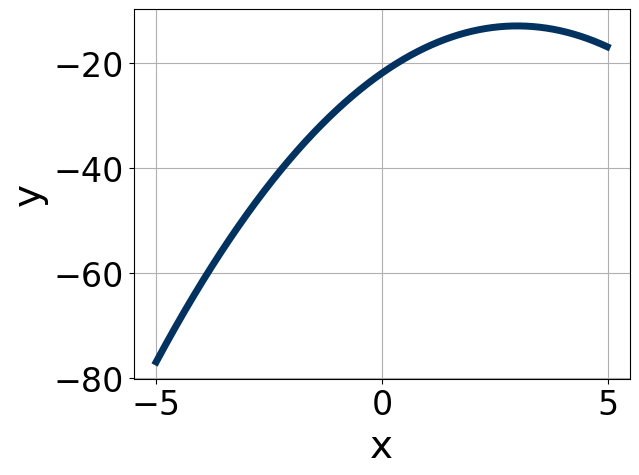
\includegraphics[width = 0.3\textwidth]{../Figures/quadraticEquationToGraphBA.png}\item 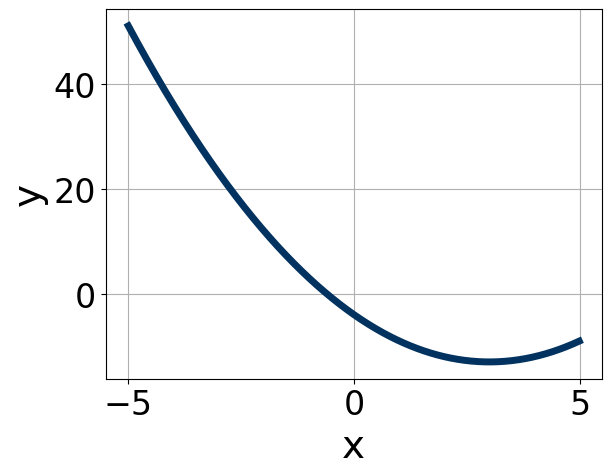
\includegraphics[width = 0.3\textwidth]{../Figures/quadraticEquationToGraphCA.png}\item 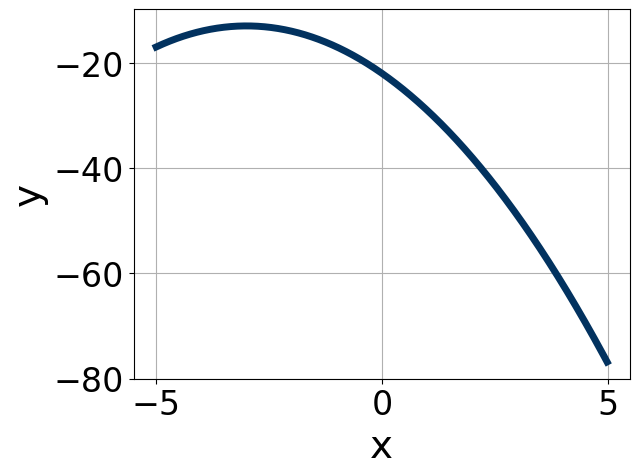
\includegraphics[width = 0.3\textwidth]{../Figures/quadraticEquationToGraphDA.png}\end{multicols}\item None of the above.
\end{enumerate} }
\end{enumerate}

\end{document}